\documentclass{article}
\usepackage{graphicx}
\usepackage{float}
\usepackage[spanish]{babel}
\usepackage{hyperref}
\usepackage{csquotes}
\graphicspath{ {img/} }
\setlength{\parskip}{\baselineskip}

\title{Patrones de Diseño: Factory Method \\[3ex] \small PAMN - Programación de Aplicaciónes Moviles Nativas}

\author{Chamil José Cruz Razeq}

\begin{document}
    \maketitle
    \thispagestyle{empty}
    \newpage

    \section{Introducción}
        Todas las tareas propuestas se encuentran disponibles en el siguiente
         repositorio de \href{https://github.com/chamilstudy/ulpgc_pamn_assigments}{GitHub}.

        Para esta resolución se ha diseñado una estructura de clases para una
         aplicación de notas en Kotlin utilizando el patrón Factory Method \cite{FactoryMethod}.

        \section{Diagrama de Clases}

        Para el diseño del programa se ha utilizado como referencia el diagrama [ Figura \ref{fig:example} ].

        \begin{figure}[H]
            \centerline{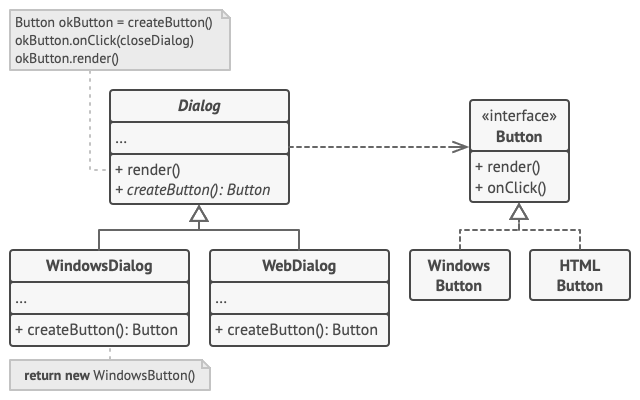
\includegraphics[scale=0.3]{example.png}}
            \caption{Diagrama de clases de aplicación de ejemplo de www.refactoring.com \cite{FactoryMethod}}
            \label{fig:example}
        \end{figure}

        Se ha replicado la estructura, siguiendo las funcionalidades propuestas en el enunciado,
         dando como resultado al diagrama [ Figura \ref{fig:uml} ]

        \begin{figure}[H]
            \centerline{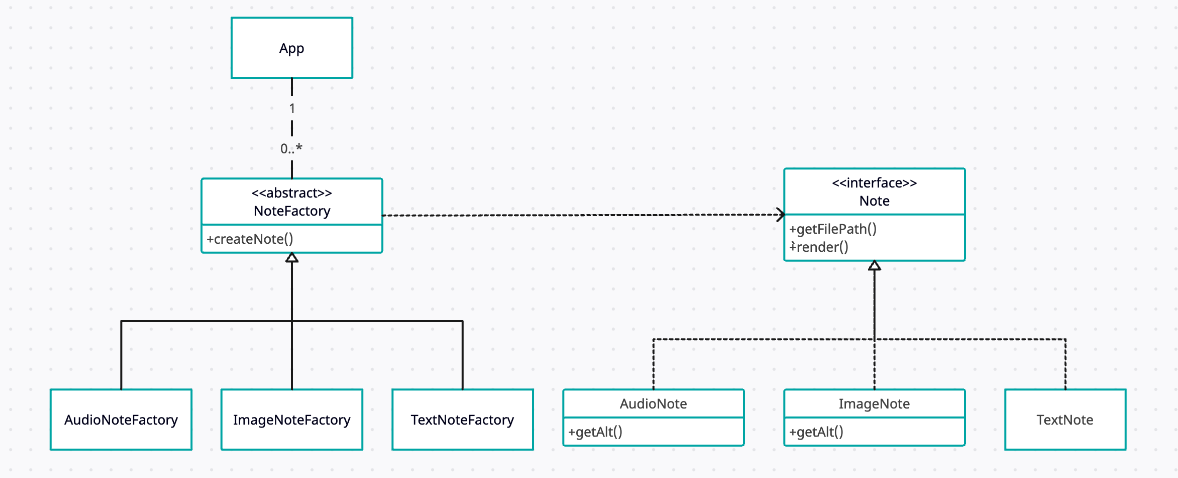
\includegraphics[scale=0.3]{uml.png}}
            \caption{Diagrama de clases de aplicación de notas}
            \label{fig:uml}
        \end{figure}

    \section{Código de Prueba}

        Se ha elaborado un pequeño programa de prueba siguiendo la estructura planteada en elaborado
         diagrama de clases. Para ello se ha utilizado el lenguaje de programación "Kotlin" y para
         ejecutarlo el laboratorio de pruebas online ofrecido por "Google".

        Comenzamos con la interfaz "Note" que servirá como abstracción de todos los tipos de
         notas de nuestro programa:

        \begin{figure}[H]
            \centerline{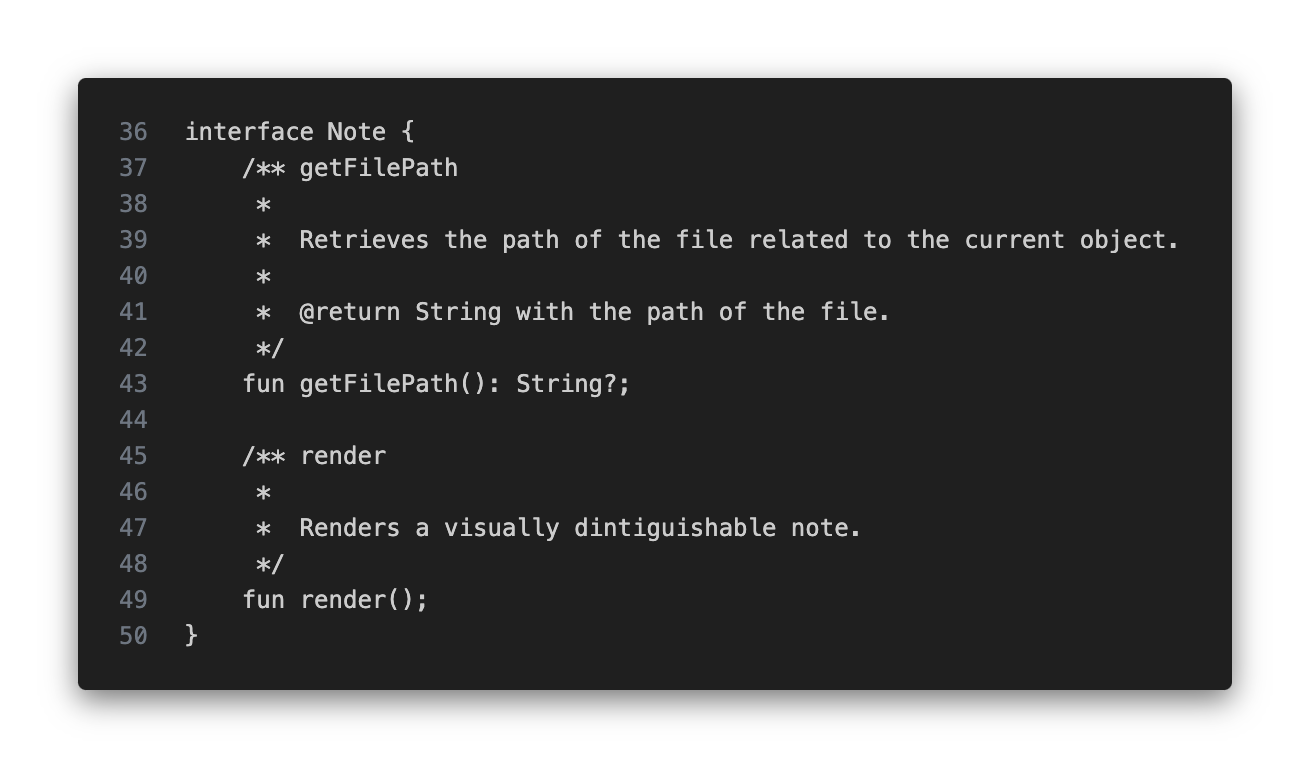
\includegraphics[scale=0.3]{note.png}}
            \caption{Interfaz de nota}
            \label{fig:note}
        \end{figure}

        Seguidamente se implementó utilizando la interfaz anterior los tres tipos de notas,
         desarrollando asimísmo sus peculiaridades, tales como "getAlt" mas afín a elementos
         audiovisuales:

        \begin{figure}[H]
            \centerline{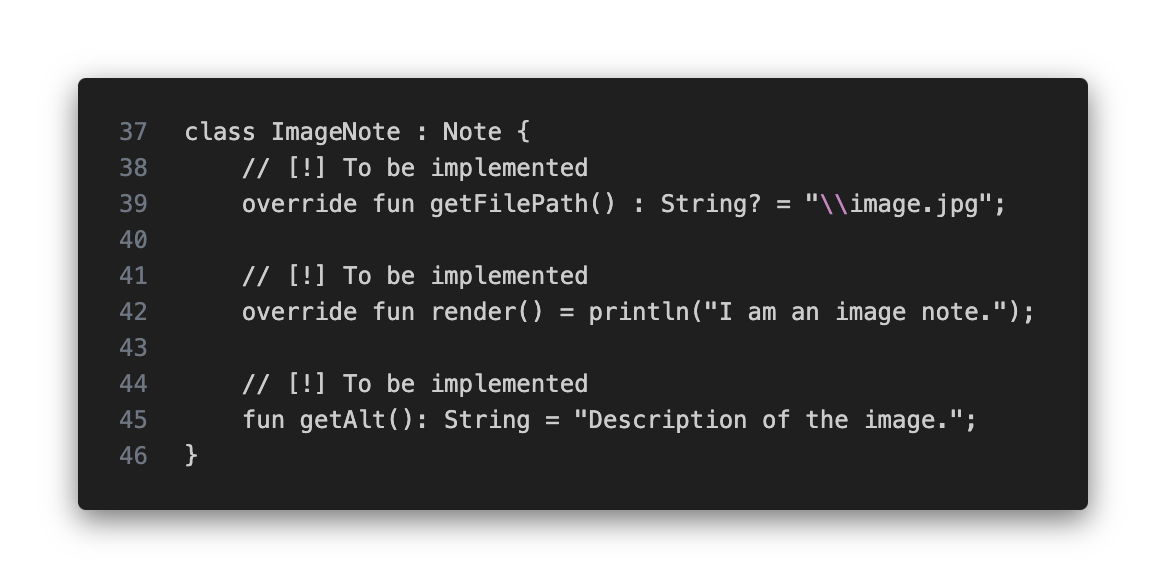
\includegraphics[scale=0.3]{image_note.png}}
            \caption{Implementación de nota de imagen}
            \label{fig:image_note}
        \end{figure}

        \begin{figure}[H]
            \centerline{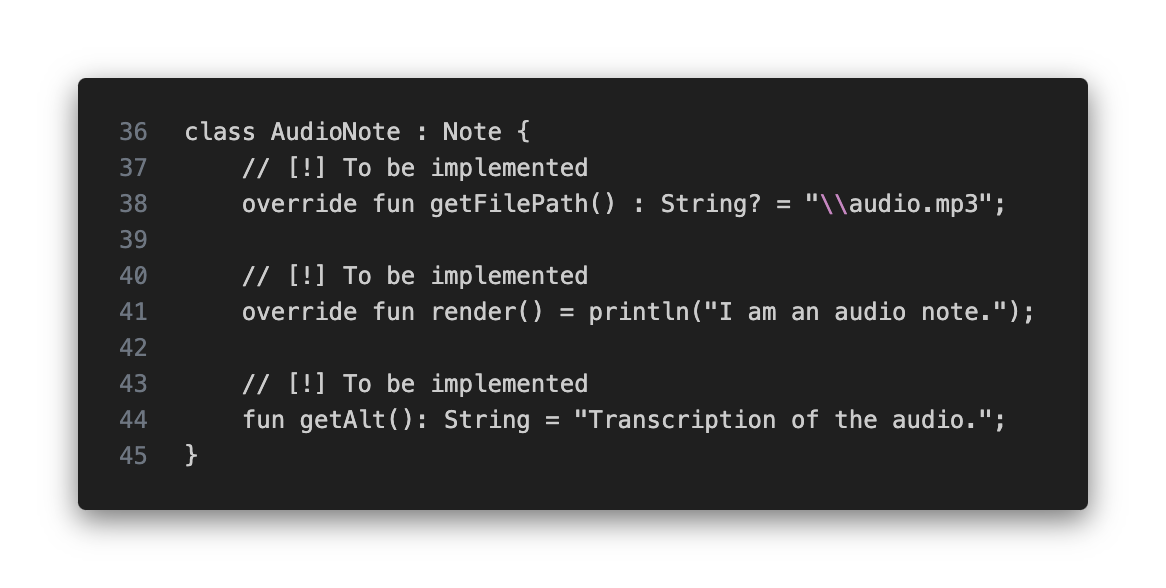
\includegraphics[scale=0.3]{audio_note.png}}
            \caption{Implementación de nota de audio}
            \label{fig:audio_note}
        \end{figure}

        \begin{figure}[H]
            \centerline{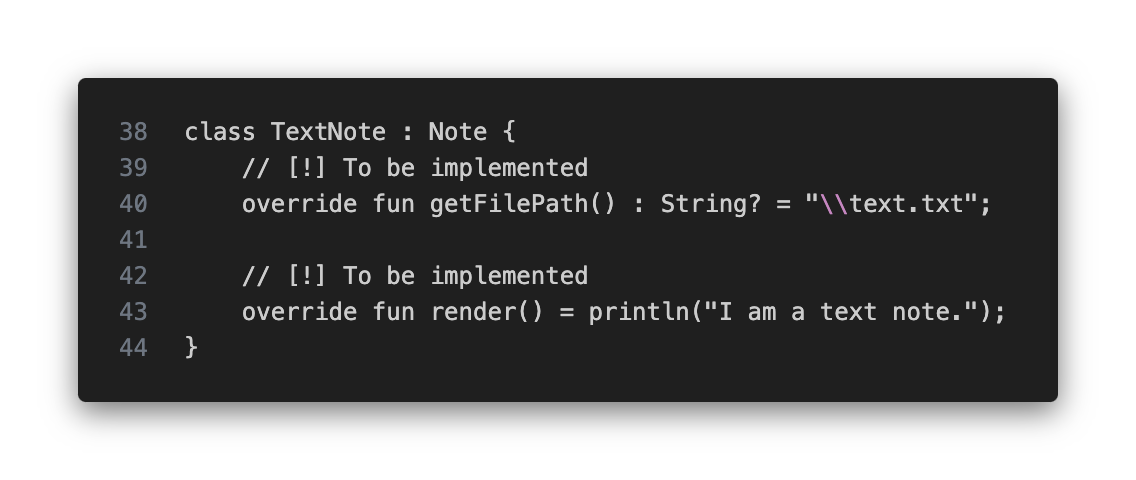
\includegraphics[scale=0.3]{text_note.png}}
            \caption{Implementación de nota de texto}
            \label{fig:text_note}
        \end{figure}

        Por otro lado se creó la clase abstracta de "producción", que servirá como abstracción
         de las clases productoras respectivas a cada clase creada anteriormente:

        \begin{figure}[H]
            \centerline{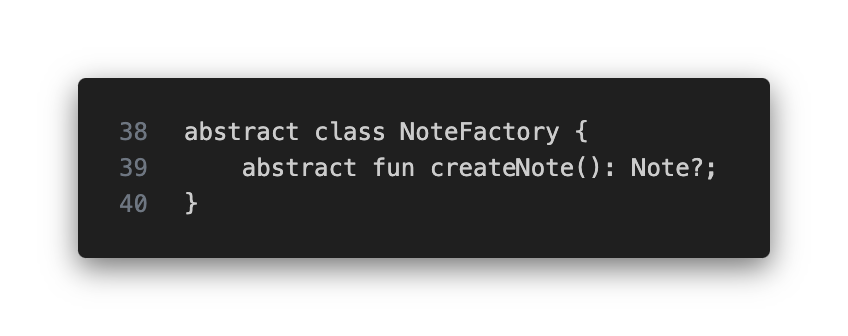
\includegraphics[scale=0.3]{note_factory.png}}
            \caption{Clase abstracta de productor de notas}
            \label{fig:note_factory}
        \end{figure}

        Como era de esperar, se desarrolló una clase productora por cada clase "Nota",
         cumpliendose así finalmente el patrón "Factory Method":

        \begin{figure}[H]
            \centerline{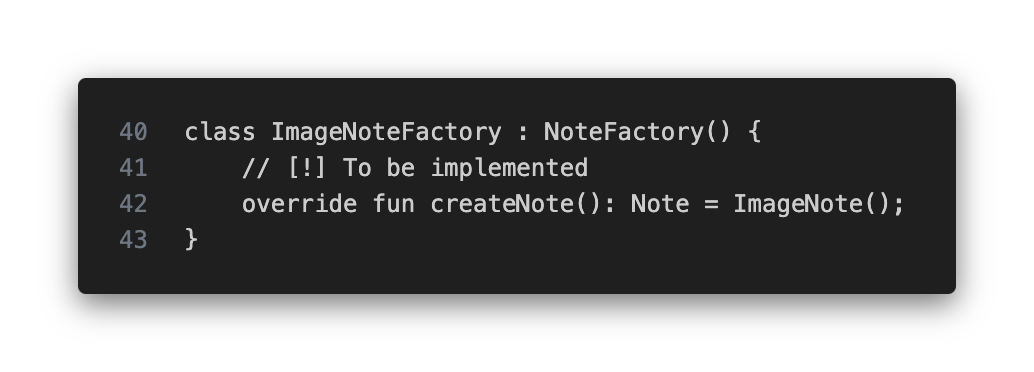
\includegraphics[scale=0.3]{image_note_factory.png}}
            \caption{Clase productora de notas de imagen}
            \label{fig:image_note_factory}
        \end{figure}

        \begin{figure}[H]
            \centerline{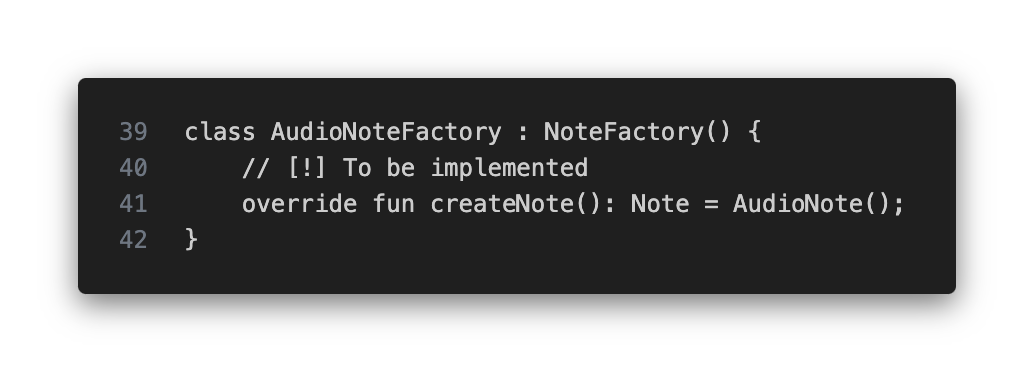
\includegraphics[scale=0.3]{audio_note_factory.png}}
            \caption{Clase productora de notas de audio}
            \label{fig:audio_note_factory}
        \end{figure}

        \begin{figure}[H]
            \centerline{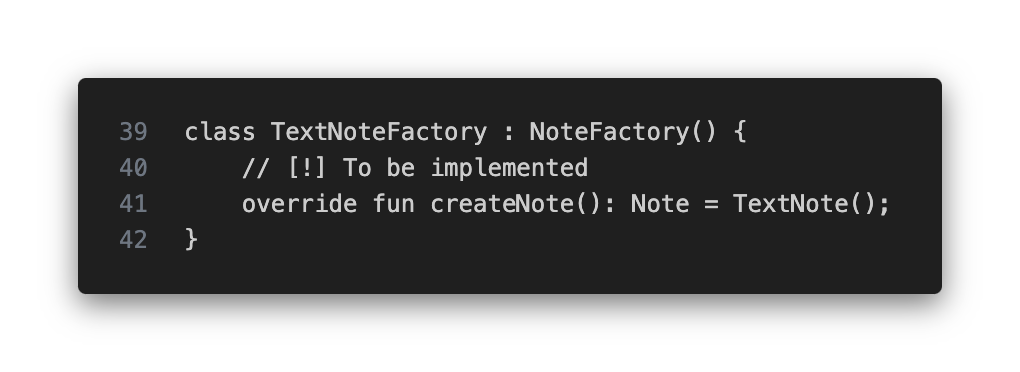
\includegraphics[scale=0.3]{text_note_factory.png}}
            \caption{Clase productora de notas de texto}
            \label{fig:text_note_factory}
        \end{figure}

    \section{Reflexión}
    Este patrón resulta útil ante la incertidumbre de la escalabilidad del código.
    
    Por un lado, al abstraer las características comunes de las "Notas" podemos garantizar la
     facilidad de incrementar el número de tipo de notas, además de promover el polimorfismo.

    Cabe destacar que, abstrayendo la producción conseguimos el mismo efecto anteriormente mencionado,
     sumando ciertas ventajas en cuanto al control y la escalabilidad de la producción.
    
    En resumidas cuentas, esta estructura facilita el despliegue de nuevas características con
     la sencilla intervención de crear una nueva clase productora y tipo, siguiendo respectivamente
     lo estipulado por la clase abstracta y interfáz.

    \begin{thebibliography}{}
        \bibitem{lab3} PAMN Lab3 Arquitectura
        \bibitem{RoomsVSSQLite} Rooms - https://medium.com/dvt-engineering/android-room-versus-sqlite-which-is-best-32ff651bc361
        \bibitem{FactoryMethod} Factory Method - https://refactoring.guru/es/design-patterns/factory-method
    \end{thebibliography}
        
\end{document}